\clearpage
\Question[2]{Pointer Illustration}\TAGS{aliasing, memory-model, pointer}

Clearly and carefully illustrate the contents of memory after the
following code runs. We've drawn the contents of \lstinline'w', a pointer
that points into allocated memory where the number 0 is stored.

\smallskip
\begin{lstlisting}
int* w = alloc(int);
int i = 12;
int* p = alloc(int);
int* q = p;
int* r = alloc(int);
int** x = alloc(int*);
int** y = alloc(int*);
int** z = y;
*r = i + 4;
*y = q;
**z = 4;
*x = r;
q = NULL;
i = *p + **y;
\end{lstlisting}

\begin{framed}
\ifprintanswers{\color{\answerColor}
\begin{lstlisting}[aboveskip=0pt, belowskip=0pt, lineskip=-0.2ex]
    ___      ___
   |   |    |   |
 w | *----->| 0 |
   |___|    |___|
   |   |
 i | 8 |
   |___|
   |   |     ____
 p | *--\   |    |
   |___| \->| 4  |<-\
   |   |    |____|   |
 q | *--||   ____    |
   |___|    |    |   |
   |   | /->| 16 |   |
 r | *--/   |____|   |
   |___|      ^      |
   |   |     _|_     |
 x | *--\   | | |    |
   |___| \->| * |    |
   |   |    |___|    |
 y | *--\    ___     |
   |___| \->|   |    |
   |   | /->| *-----/
 z | *--/   |___|
   |___|
\end{lstlisting}
}\else
  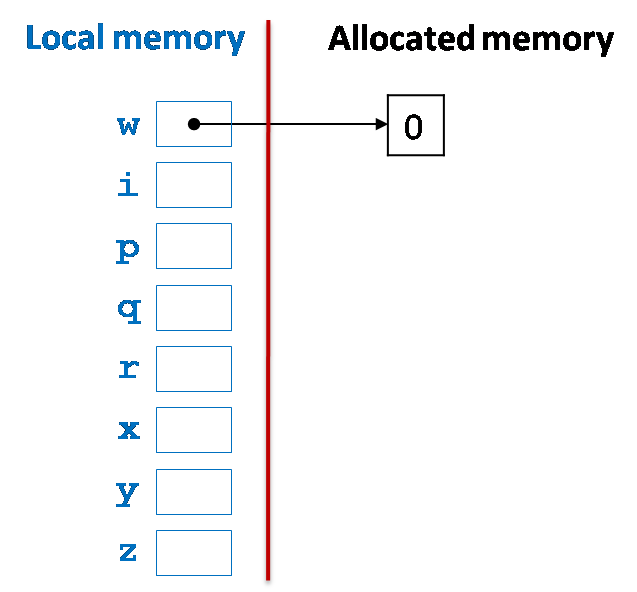
\includegraphics[width=0.82\textwidth]{\img/template.png}
\fi
\end{framed}

\RUBRIC
TAGS: aliasing, memory-model, pointer

Gradescope rubric:
+ 1 pt i, *p, and *r are 8, 4, and 16, respectively
+ 1 pt r == *x, y == z, *y == p

Commentary:
    ___      ___
   |   |    |   |
 w | *----->| 0 |
   |___|    |___|
   |   |
 i | 8 |
   |___|
   |   |     ____
 p | *--\   |    |
   |___| \->| 4  |<-\
   |   |    |____|   |
 q | *--||   ____    |
   |___|    |    |   |
   |   | /->| 16 |   |
 r | *--/   |____|   |
   |___|      ^      |
   |   |     _|_     |
 x | *--\   | | |    |
   |___| \->| * |    |
   |   |    |___|    |
 y | *--\    ___     |
   |___| \->|   |    |
   |   | /->| *-----/
 z | *--/   |___|
   |___|

1 point
  . i, *p, and *r return the correct answers, q is NULL
  . All or nothing (this was easy for them to test)
1 point - Structure is correct: p == q, y == z, *x == r, *y == p
  . Half of this point if no more than two structure arrows are wrong
ENDRUBRIC
